%%%%%%%%%%%%%%%%%%%%% chapter.tex %%%%%%%%%%%%%%%%%%%%%%%%%%%%%%%%%
%
% sample chapter
%
% Use this file as a template for your own input.
%
%%%%%%%%%%%%%%%%%%%%%%%% Springer-Verlag %%%%%%%%%%%%%%%%%%%%%%%%%%
%\motto{Use the template \emph{chapter.tex} to style the various elements of your chapter content.}
\chapter{Example B: single sector economy with external demand}
\chaptermark{Example B}
\label{chap:single_sector_ext_demand} % Always give a unique label
% use \chaptermark{}
% to alter or adjust the chapter heading in the running head

\abstract*{[NEED TO ADD ABSTRACT HERE]}

%% \abstract{Each chapter should be preceded by an abstract (10--15 lines long) that summarizes the content. The abstract will appear \textit{online} at \url{www.SpringerLink.com} and be available with unrestricted access. This allows unregistered users to read the abstract as a teaser for the complete chapter. As a general rule the abstracts will not appear in the printed version of your book unless it is the style of your particular book or that of the series to which your book belongs.\newline\indent
%% Please use the 'starred' version of the new Springer \texttt{abstract} command for typesetting the text of the online abstracts (cf. source file of this chapter template \texttt{abstract}) and include them with the source files of your manuscript. Use the plain \texttt{abstract} command if the abstract is also to appear in the printed version of the book.}

%% Use the template \emph{chapter.tex} together with the Springer document class SVMono (monograph-type books) or SVMult (edited books) to style the various elements of your chapter content in the Springer layout.


At this point, we move to a second example wherein a single economic sector (3) interacts with Society (2, which provides final demand) and the Earth (1, the destination for waste heat and the source of all resources). In this economy, we assume that the purpose of the goods and services sector is to produce goods and provide services, including the provision of direct energy available to the economy and society.

%%%%%%%%%% Example B %%%%%%%%%%
\section{First Law of Thermodynamics}
%%%%%%%%%%

The First Law of Thermodynamics requires that energy (direct and waste heat) is conserved around each Sector of the economy (3) as well as around the Earth (1) and Society (2) as shown in Figure \ref{fig:direct_energy_flows}. 

\begin{figure}[h!]
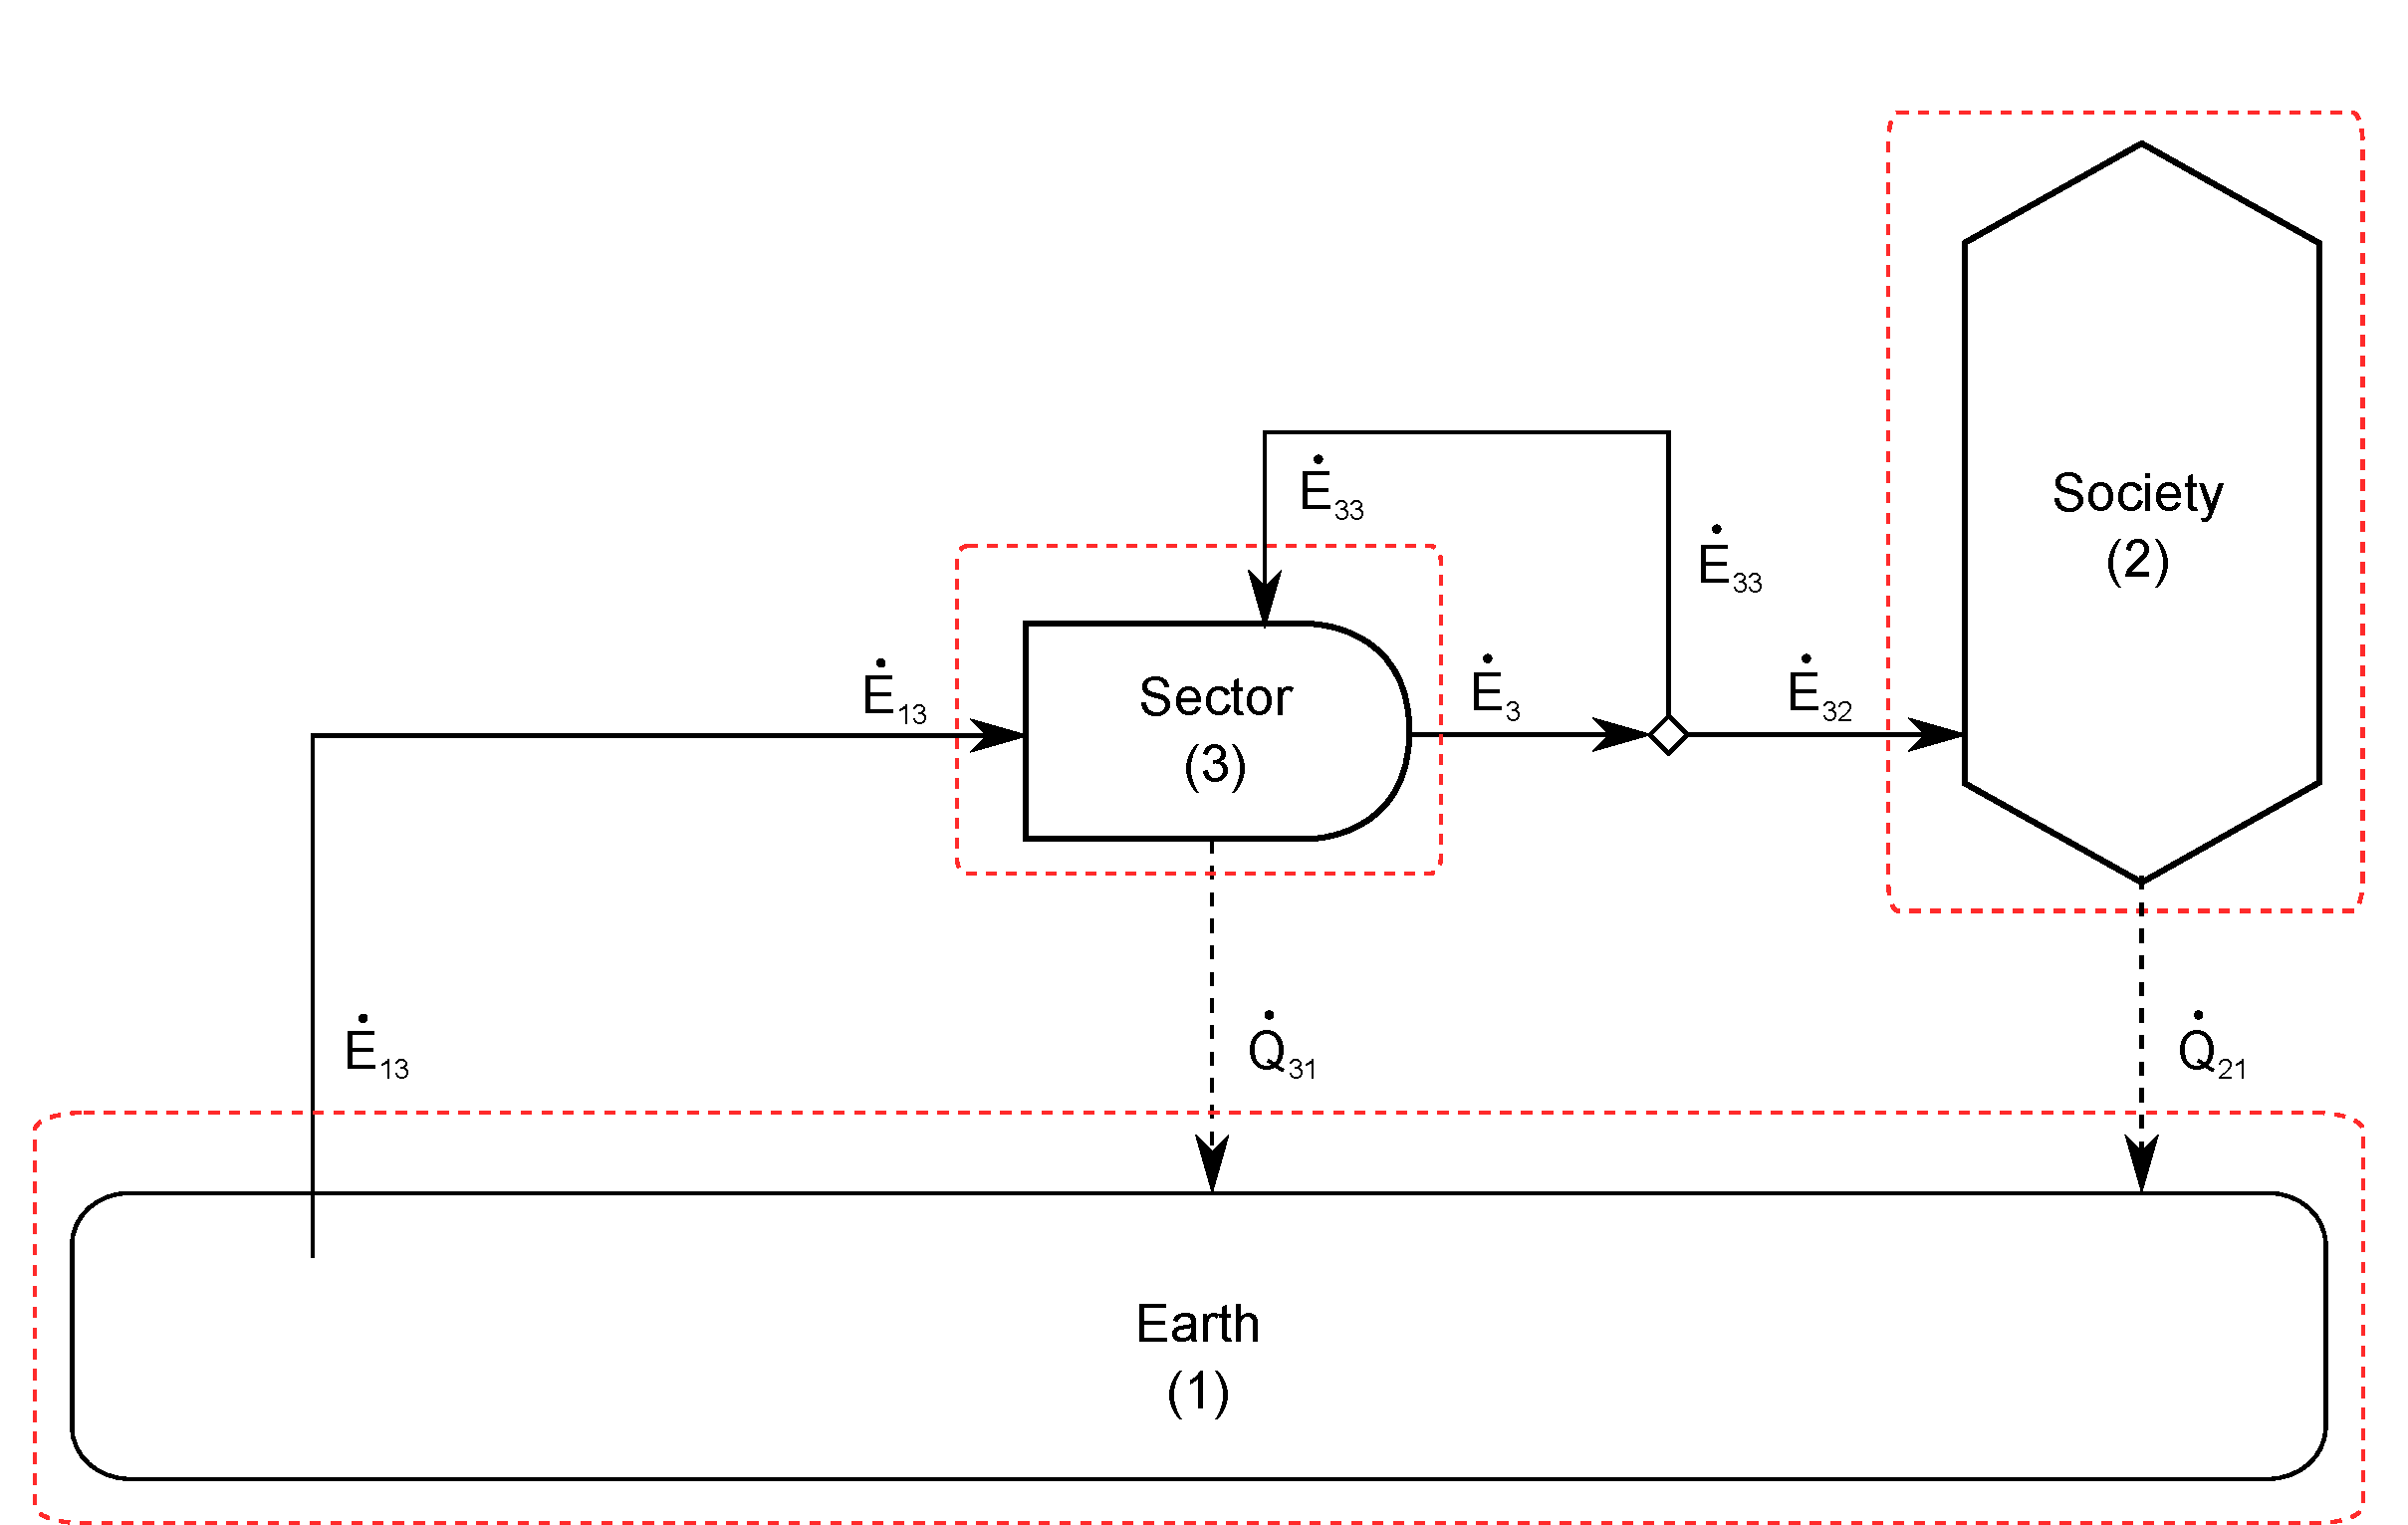
\includegraphics[width=1.0\linewidth]{Chapter_Example_B/images/I-O_two_sector_direct_energy.pdf}
\caption{Flows of direct energy ($\dot{E}$) and waste heat ($\dot{Q}$) in a one-sector economy with separate demand.}
\label{fig:direct_energy_flows}
\end{figure}

The First Law around the economic Sector (3) including the accumulation rate of direct energy in the sector $\left(\frac{\mathrm{d}E_{3}}{\mathrm{d}t}\right)$ yields

\begin{equation} \label{eq:CV_E_dot_3}
	\frac{\mathrm{d}E_{3}}{\mathrm{d}t} 	 = \dot{E}_{13} + \dot{E}_{33} - \dot{E}_{3} - \dot{Q}_{31}.
\end{equation}

\noindent It is notable that the economic Sector (3) consumes a portion of its own energy output ($\dot{E}_{33}$) as it produces its goods and services: it takes energy to make energy.

First Law energy accounting around the Earth (1) and Society (2) gives

\begin{equation} \label{eq:CV_E_dot_1}
	\frac{\mathrm{d}E_{1}}{\mathrm{d}t} 	 =  \dot{Q}_{21} + \dot{Q}_{31} - \dot{E}_{13},
\end{equation}

\noindent and 

\begin{equation} \label{eq:CV_E_dot_2}
	\frac{\mathrm{d}E_{2}}{\mathrm{d}t} 	 = \dot{E}_{32} - \dot{Q}_{21}.
\end{equation}

As in Example A, we can set the accumulation of direct energy within each sector to zero to obtain

\begin{equation} \label{eq:CV_E_dot_3_SS}
	0 =\dot{E}_{13} + \dot{E}_{33} - \dot{E}_{3} - \dot{Q}_{31},
\end{equation}

\begin{equation} \label{eq:CV_E_dot_1_SS}
	0 =  \dot{Q}_{21} + \dot{Q}_{31} - \dot{E}_{13},
\end{equation}

\noindent and 

\begin{equation} \label{eq:CV_E_dot_2_SS}
	0 =\dot{E}_{32} - \dot{Q}_{21},
\end{equation}

%%%%%%%%%%% Example B %%%%%%%%%%
%\section{Energy ratios}
%%%%%%%%%%%
%
%[IS THERE ANY POINT IN DEFINING THESE HERE IF THEY ARE NOT USED? I HAVE COMMENTED THEM OUT AS I THINK THEY HAVE BEEN MOVED TO LATER SECTION IN EXAMPLE C - MD]
%
%Several important energy ratios can be observed in Figure \ref{fig:direct_energy_flows}. The Gross Energy Ratio ($GER$) is defined as 
%
%\begin{equation} \label{eq:GER_def_ch_5}
%	GER \equiv \frac{\dot{E}_{3}}{\dot{E}_{33}}.
%\end{equation}
%
%\noindent The Net Energy Ratio ($NER$) is defined as
%
%\begin{equation} \label{eq:NER_def_ch_5}
%	NER \equiv \frac{\dot{E}_{32}}{\dot{E}_{33}} = GER - 1.
%\end{equation}
%
%[THESE DEFINITIONS ARE EQUIVALENT TO $\beta$ BOUNDARY DEFINED IN BRANDT AND DALE (2011). WE CANNOT DISTINGUISH EXTERNAL ENERGY RATIOS AT THIS POINT. NOT SURE ABOUT COMMENTED WORK BELOW - CHECK TEX FILE.]

%The rate of energy extracted from the Earth can be expressed as either
%
%\begin{equation} \label{eq:E_dot_13_a}
%	\dot{E}_{13} = \frac{GER - 1}{NEER}\dot{E}_{22}
%\end{equation}
%
%\noindent or
%
%\begin{equation} \label{eq:E_dot_32_b}
%	\dot{E}_{32} = \frac{1 - \frac{1}{GER}}{NEER}\dot{E}_{2}.
%\end{equation}

%%%%%%%%%% Example B %%%%%%%%%%
\section{Total energy accounting}
%%%%%%%%%%

Again, we follow the I-O literature in assuming that total energy (i.e., the sum of direct energy and indirect energy) is conserved. Thus, we can draw a diagram similar to Figure \ref{fig:direct_energy_flows} for total energy flows. See Figure \ref{fig:total_energy_flows_1S}.

\begin{figure}[h!]
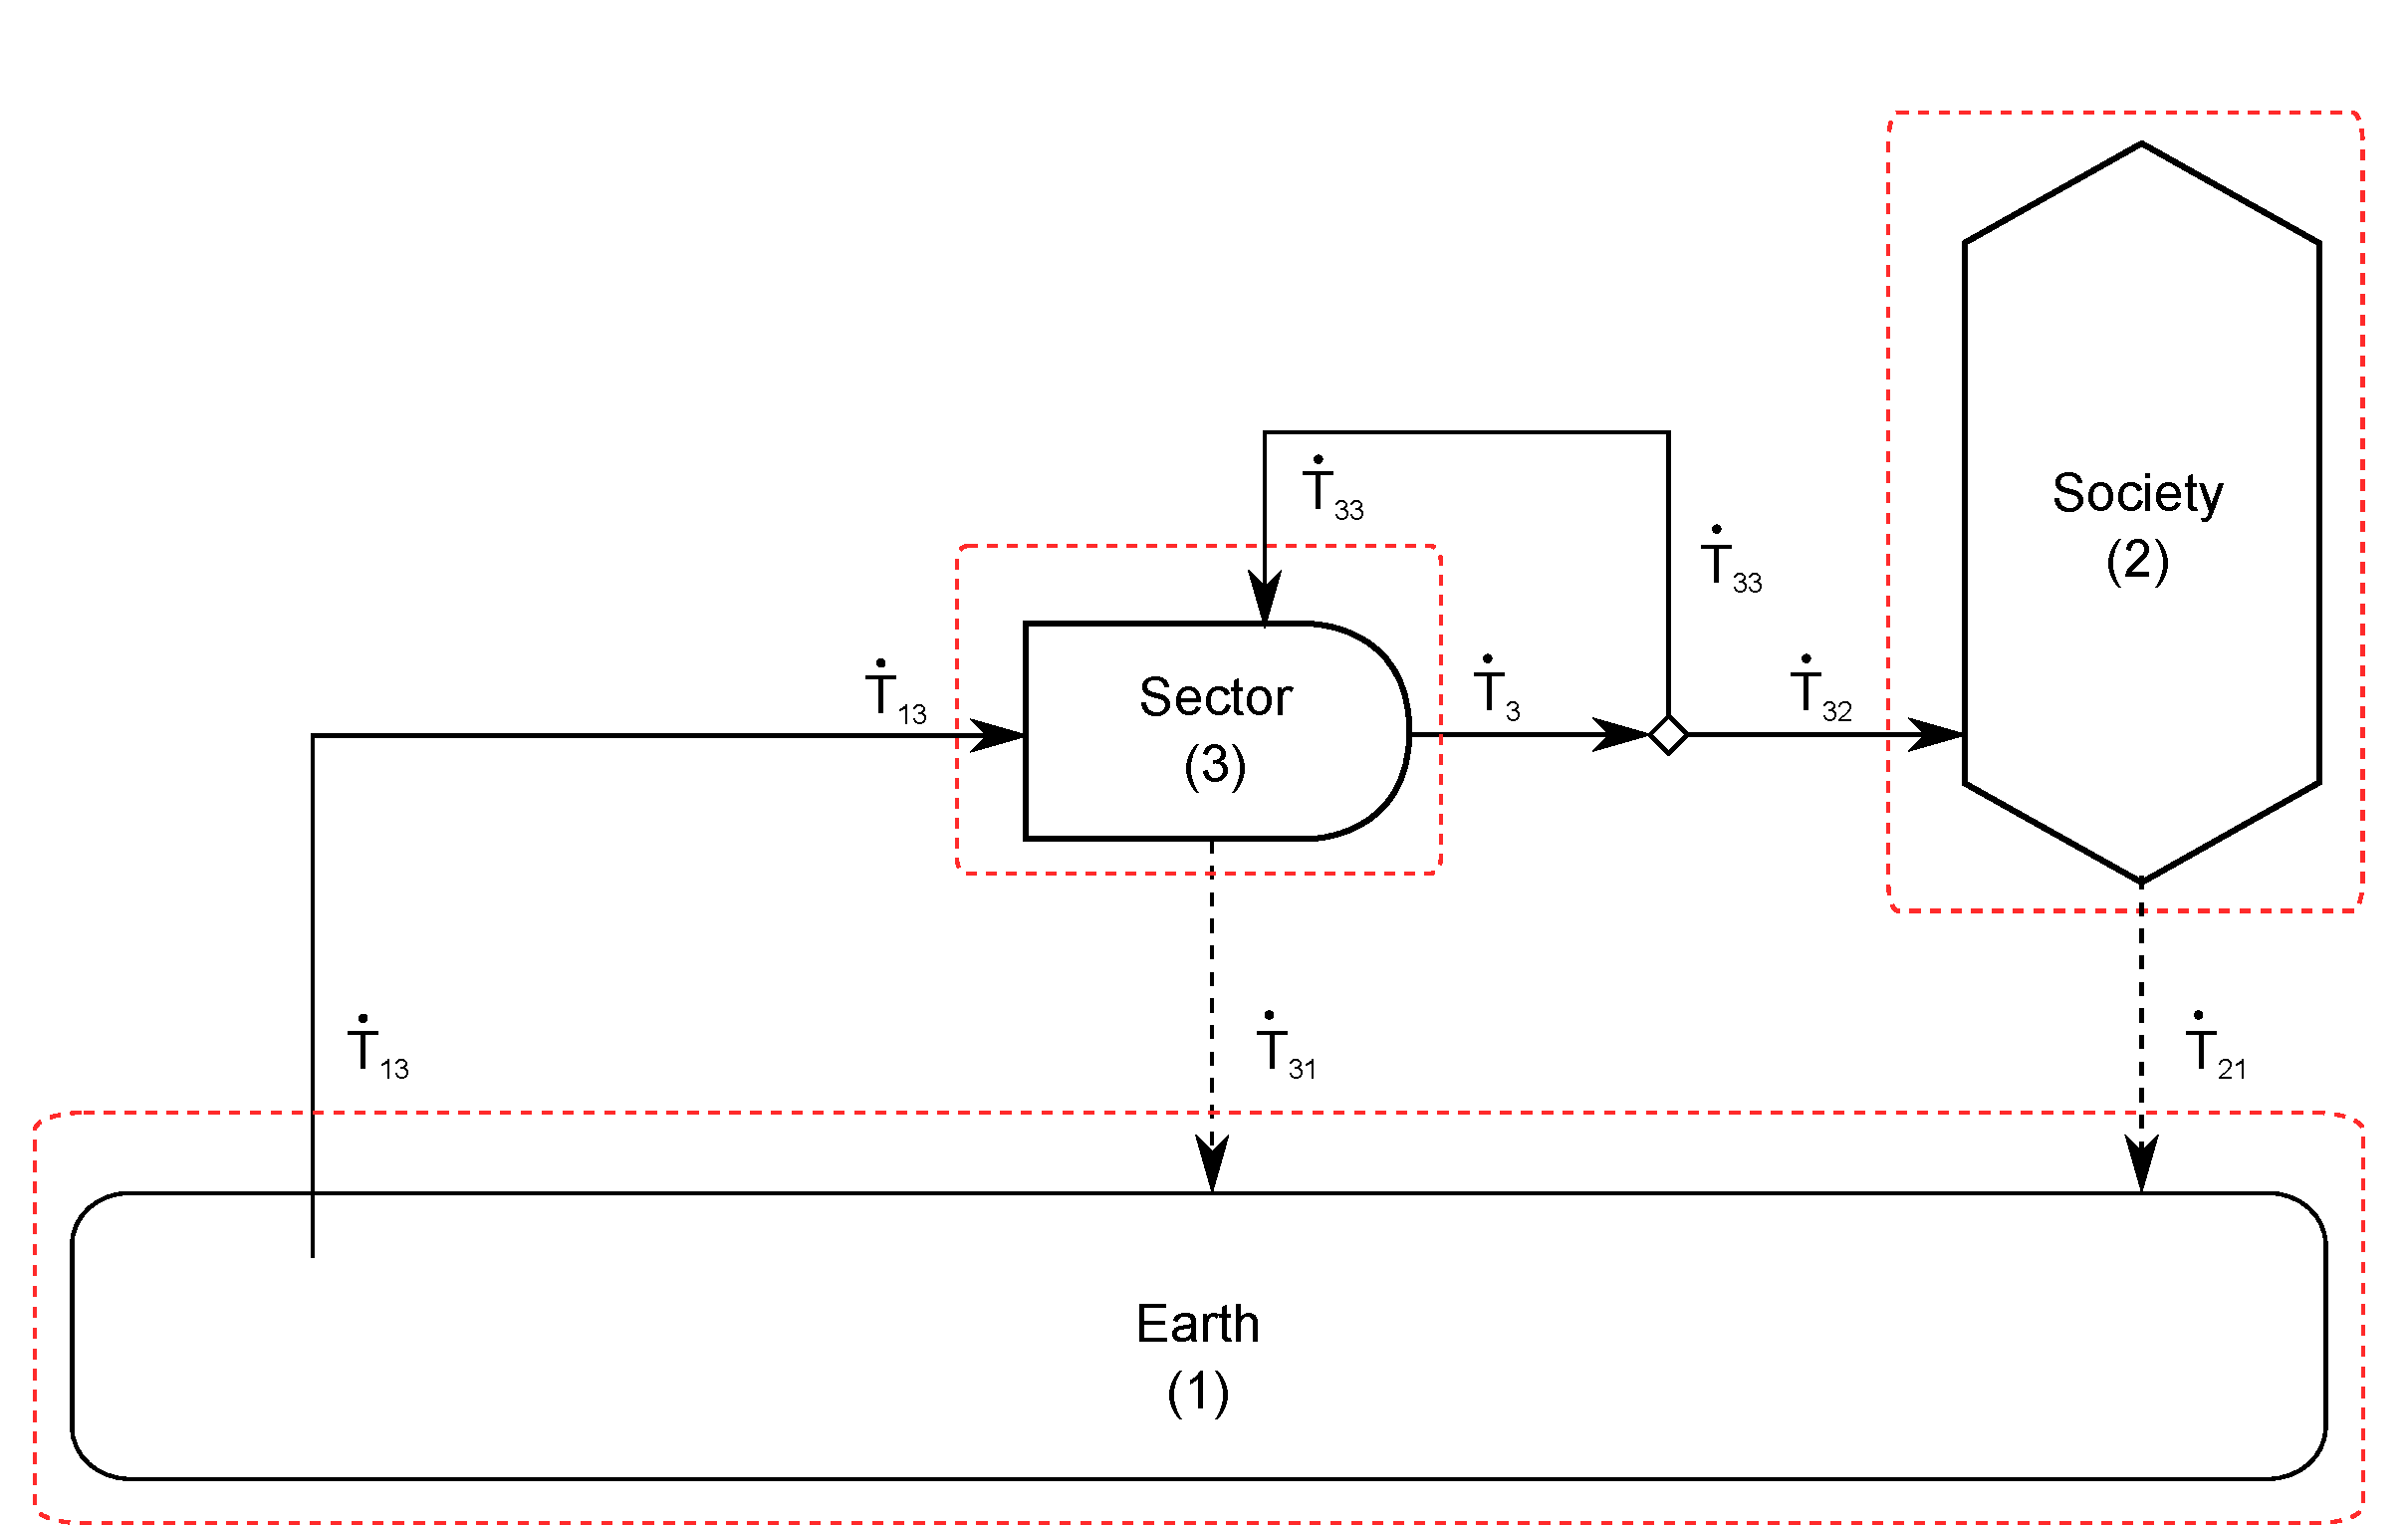
\includegraphics[width=1.0\linewidth]{Chapter_Example_B/images/I-O_two_sector_total_energy.pdf}
\caption{Flows of total energy ($\dot{T}$) in a one-sector economy with separate demand.}
\label{fig:total_energy_flows_1S}
\end{figure}

Accounting for accumulation of total energy and using the assumption that total energy is conserved, we can write the following equations.

\begin{equation} \label{eq:CV_T_1}
	\frac{\mathrm{d}T_{1}}{\mathrm{d}t} 	 = \dot{T}_{21} + \dot{T}_{31} - \dot{T}_{13},
\end{equation}

\begin{equation} \label{eq:CV_T_2}
	\frac{\mathrm{d}T_{2}}{\mathrm{d}t} 	 = \dot{T}_{32} - \dot{T}_{21},
\end{equation}

\noindent and

\begin{equation} \label{eq:CV_T_3}
	\frac{\mathrm{d}T_{3}}{\mathrm{d}t} 	 = \dot{T}_{13} + \dot{T}_{33} - \dot{T}_{3} - \dot{T}_{31}.
\end{equation}

%%%%%%%%%% Example B %%%%%%%%%%
\section{Embodied energy accounting}
%%%%%%%%%%

Given that $\frac{\mathrm{d}E_{i}}{\mathrm{d}t} = 0$ and $\dot{T} = \dot{E} + \dot{B}$, we note that

\begin{equation} \label{eq:T_dot_equals_B_dot}
	\frac{\mathrm{d}T_i}{\mathrm{d}t} = \frac{\mathrm{d}B_i}{\mathrm{d}t},
\end{equation}

\noindent and we can rewrite the total energy accumulation accounting equations as

\begin{equation} \label{eq:CV_dB_1}
	\frac{\mathrm{d}B_{1}}{\mathrm{d}t} = \dot{E}_{21} + \dot{B}_{21} + \dot{E}_{31} + \dot{B}_{31} - \dot{E}_{13} + \dot{B}_{13},
\end{equation}

\begin{equation} \label{eq:CV_dB_2}
	\frac{\mathrm{d}B_{2}}{\mathrm{d}t} = \dot{E}_{32} + \dot{B}_{32} - \dot{E}_{21} - \dot{B}_{21},
\end{equation}

\noindent and 

\begin{equation} \label{eq:CV_dB_3}
	\frac{\mathrm{d}B_{3}}{\mathrm{d}t} = \dot{E}_{13} + \dot{B}_{13} + \dot{E}_{33} + \dot{B}_{33} - \dot{E}_{3} - \dot{B}_{3} - \dot{E}_{31} - \dot{B}_{31}.
\end{equation}

As in Example A, we can substitute the First Law of Thermodynamics for the economic Sector (Equation \ref{eq:CV_E_dot_3_SS}) into the total energy accounting equation for the economic Sector (Equation \ref{eq:CV_dB_3}). Assuming that $\dot{E}_{31} = 0$ (because energy is returned to the Earth as waste heat, not direct energy), we obtain

\begin{equation} \label{eq:ExB_embodied_energy_accounting}
	\frac{\mathrm{d}B_3}{\mathrm{d}t} = \dot{Q}_{31} + \dot{B}_{13} + \dot{B}_{33} - \dot{B}_{31}
\end{equation}

Similar to Example A, we observe that the accumulation rate of embodied energy in the Goods and Services sector (3) is the sum of the rates of waste heat from the sector ($\dot{Q}_{31}$) and embodied energy into the sector ($\dot{B}_{13} + \dot{B}_{33}$) less the rate of embodied energy leaving the sector on its output stream ($\dot{B}_{31}$).

%%%%%%%%%% Example B %%%%%%%%%%
\section{Depreciation}
%%%%%%%%%%

We can substitute a depreciation term for the flow rate of embodied energy from the economic Sector (3) to the Earth (1) to obtain

\begin{equation} \label{eq:ExB_embodied_energy_accounting_with_depreciation}
	\frac{\mathrm{d}B_3}{\mathrm{d}t} = \dot{Q}_{31} + \dot{B}_{13} + \dot{B}_{33} - \gamma_3 B_3.
\end{equation}

%%%%%%%%%% Example B %%%%%%%%%%
\section{Estimating energy intensity ($\varepsilon$) of the economy}
%%%%%%%%%%

The following figure shows value flows ($\dot{X}$) in the one-sector economy with separate demand.

\begin{figure}[H]
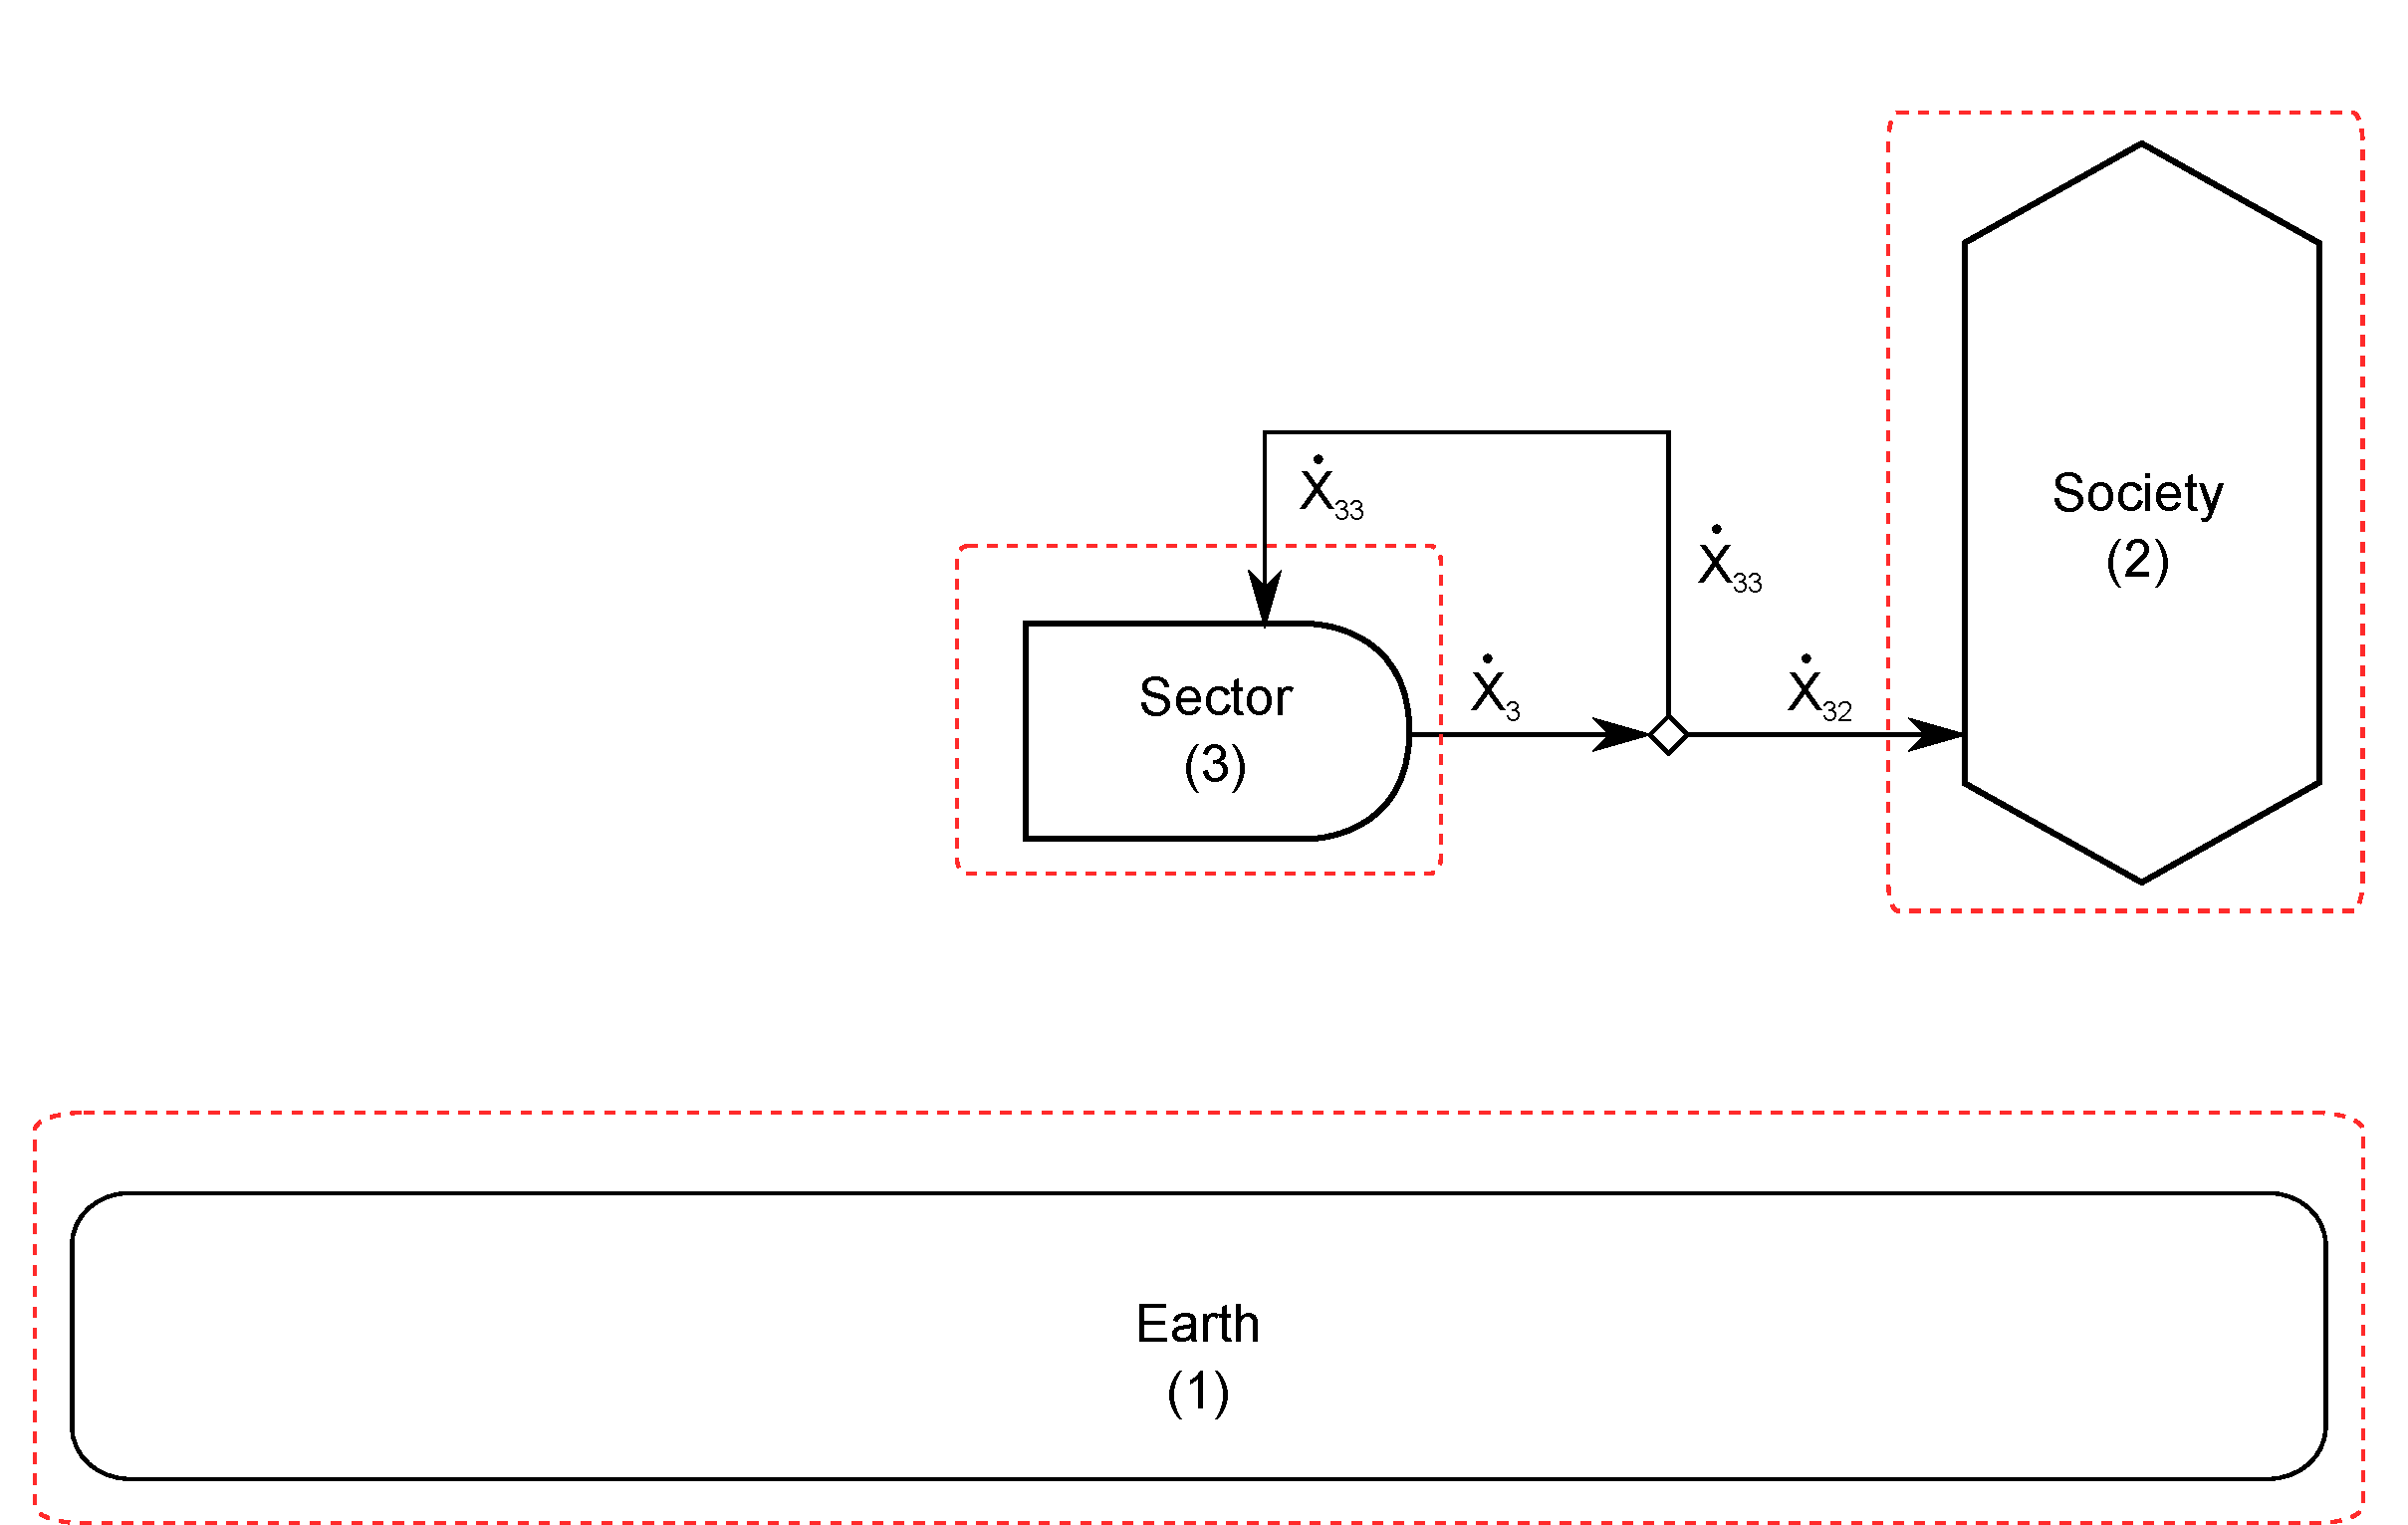
\includegraphics[width=1.0\linewidth]{Chapter_Example_B/images/I-O_two_sector_value.pdf}
\caption{Flows of economic value ($\dot{X}$) in a one-sector economy with separate demand.}
\label{fig:economic_value_flows}
\end{figure}

The energy intensity ($\varepsilon$) of the economic Sector (3) is given by

\begin{equation} \label{eq:single_sector_energy_intensity}
	\varepsilon_{3} = \frac{\dot{T}_{3}}{\dot{X}_{3}} = \frac{\dot{T}_{33}}{\dot{X}_{33}}.
\end{equation}

The input-output ratio ($a$) for the economic Sector (3) is

\begin{equation} \label{eq:io_ratio_single_sector}
	a_{33} = \frac{\dot{X}_{33}}{\dot{X}_{3}}.
\end{equation}

\noindent Thus,

\begin{equation} \label{eq:T_dot_1_single_sector}
	\dot{T}_{3} = \varepsilon_{3}\dot{X}_{3},
\end{equation}

\noindent and

\begin{equation} \label{eq:T_dot_11_single_sector}
	\dot{T}_{33} = \varepsilon_{3}a_{33}\dot{X}_{3}.
\end{equation}

Realizing that (a) $\frac{\mathrm{d}T_3}{\mathrm{d}t} = \frac{\mathrm{d}B_3}{\mathrm{d}t}$ because $\frac{\mathrm{d}E_3}{\mathrm{d}t} = 0$, (b) $\dot{T}_{13} = \dot{E}_{13}$ because $\dot{B}_{13} = 0$ due to processing of raw energy carriers occurring \emph{within} the economic Sector (3), and (c) substituting Equations \ref{eq:T_dot_1_single_sector} and \ref{eq:T_dot_11_single_sector} into Equation \ref{eq:CV_T_3} gives

\begin{equation} \label{eq:dB1/dt_single_sector_after_substituting_eps_and_a}
	\frac{\mathrm{d}B_{3}}{\mathrm{d}t} = \varepsilon_{3}a_{33}\dot{X}_{3} + \dot{E}_{13} - \varepsilon_{3}\dot{X}_{3} - \gamma_{3}B_{3}.
\end{equation}

We can estimate the energy intensity of the economy by solving Equation \ref{eq:dB1/dt_single_sector_after_substituting_eps_and_a} for $\varepsilon_{3}$.

\begin{equation} \label{eq:eps3_ss_IO}
	\varepsilon_{3} = (1 - a_{33})^{-1} \dot{X}_{3}^{-1} \left[\dot{E}_{13} - \left(\frac{\mathrm{d}B_{3}}{\mathrm{d}t} + \gamma_{3}B_{3}\right)\right]
\end{equation}

Equation \ref{eq:eps3_ss_IO} is similar to the typical energy intensity equation found in the I-O literature [REFERENCE BULLARD AND OTHERS HERE. --MKH], except that Equation \ref{eq:eps3_ss_IO} applies to a single economic sector and contains scalar (as opposed to matrix) terms. Using Example C below, we will derive a matrix representation of Equation \ref{eq:eps3_ss_IO} that is directly comparable to energy intensity equations found in the I-O literature.

%%%%%%%%% Example B %%%%%%%%%%
\section{Derivation of economic sector energy intensity ($\varepsilon$) by a convergent infinite series}
%%%%%%%%%%

The single-sector economy of Figures \ref{fig:direct_energy_flows} through \ref{fig:economic_value_flows} can be re-drawn as shown in Figure \ref{fig:single_sector_flows_3}.

\begin{figure}[h!]
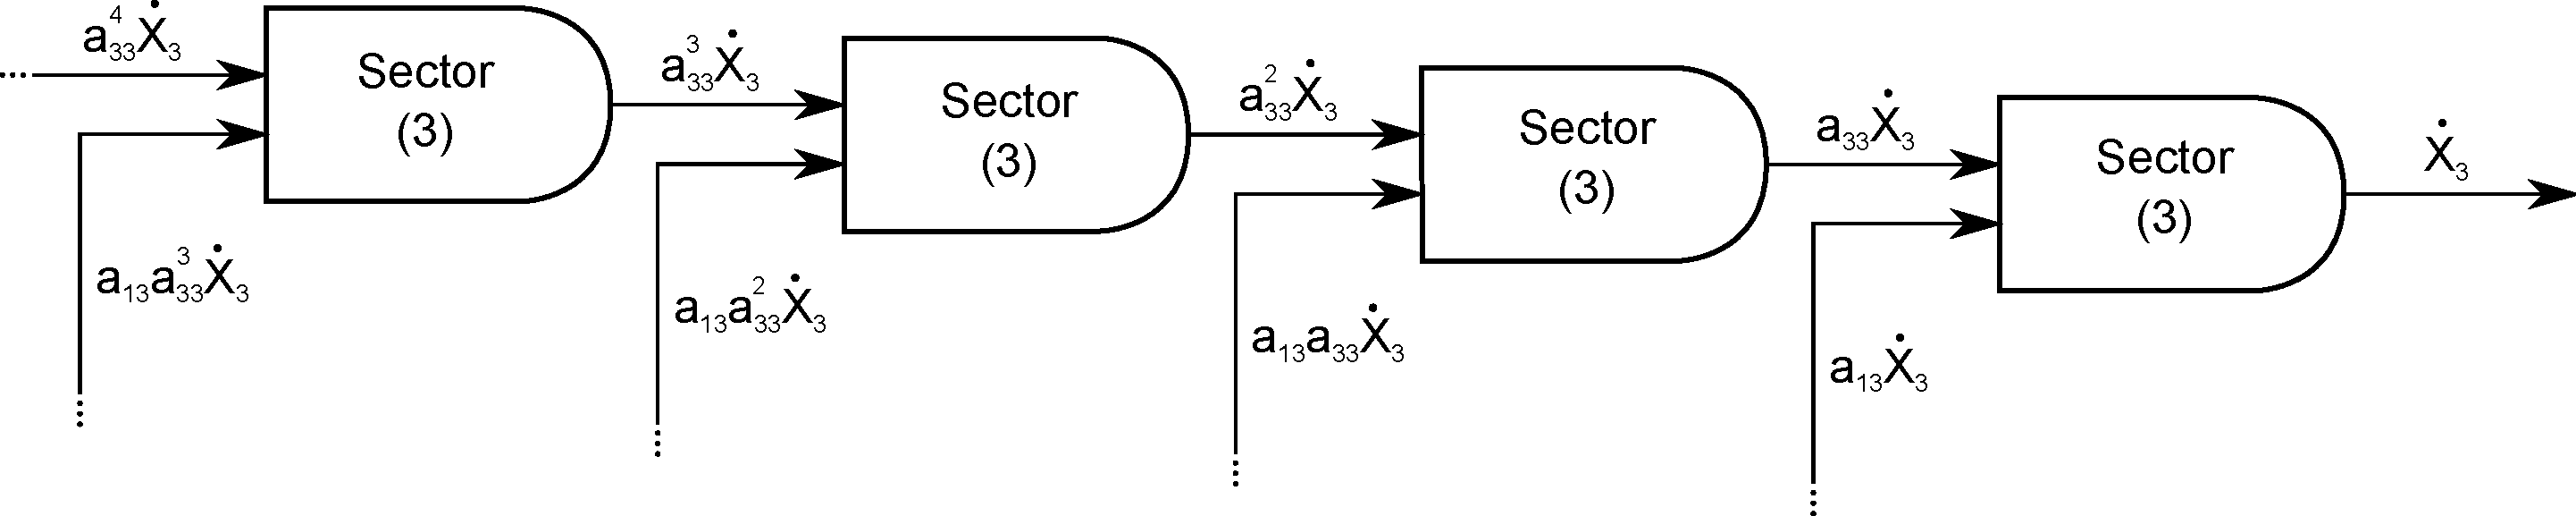
\includegraphics[width=1.0\linewidth]{Chapter_Example_B/images/Heun_I-O_Process_Equivalence_3.pdf}
\caption{Process flows in a single-sector economy.}
\label{fig:single_sector_flows_3}
\end{figure}

The economy produces output at a rate of $\dot{X}_{3}$, but it requires energy from the Earth ($\dot{E}_{13} = a_{13}\dot{X}_{3}$) to do so. The economy also consumes a fraction of its own gross output ($\dot{X}_{33} = a_{33}\dot{X}_{3}$). To produce $a_{33}\dot{X}_{3}$, the economy requires an additional $a_{13}a_{33}\dot{X}_{3}$ of energy from the Earth. The total energy required for the economy to produce at a rate of $\dot{X}_{3}$ is an infinite sum.

\begin{equation} \label{eq:E_dot_demand_SS}
	\dot{E}_{demand} = a_{13}\dot{X}_{3} + a_{13}a_{33}\dot{X}_{3} + a_{13}a_{33}^2\dot{X}_{3} + \cdots
\end{equation}

The energy intensity of the economy ($\varepsilon_{3}$) is 

\begin{equation} \label{eq:epsilon_process_SS_intermediate}
	\varepsilon_{3} = \frac{\dot{E}_{demand}}{\dot{X}_{3}} = a_{13}(1 + a_{33} + a_{33}^2) + \cdots = a_{13}\sum_{n=0}^{\infty}a_{33}^{n}.
\end{equation}

Realizing that $\sum_{n=0}^{\infty}a_{33}^{n} = \frac{1}{1-a_{33}}$ and $a_{13} = \frac{\dot{E}_{13}}{\dot{X}_{3}}$ gives

\begin{equation} \label{eq:epsilon_process_SS}
	\varepsilon_{1} = (1-a_{33})^{-1} \dot{X}^{-1} \dot{E}_{13}.
\end{equation}

Neglecting accumulation of embodied energy in the economy $\left(\frac{\mathrm{d}B_{3}}{\mathrm{d}t}\right)$ and depreciation $\left(\gamma_{3}B_{3}\right)$, Equations \ref{eq:eps3_ss_IO} and \ref{eq:epsilon_process_SS} are identical (assuming $\frac{\mathrm{d}B_{3}}{\mathrm{d}t} =\gamma_{3} = 0$), indicating that the I-O approach accounts for the infinite recursion of energy demand by the economy.




\bibliography{EROI_review_v2}
\bibliographystyle{unsrt}


% Always give a unique label
% and use \ref{<label>} for cross-references
% and \cite{<label>} for bibliographic references
% use \sectionmark{}
% to alter or adjust the section heading in the running head
%% Instead of simply listing headings of different levels we recommend to let every heading be followed by at least a short passage of text. Furtheron please use the \LaTeX\ automatism for all your cross-references and citations.

%% Please note that the first line of text that follows a heading is not indented, whereas the first lines of all subsequent paragraphs are.

%% Use the standard \verb|equation| environment to typeset your equations, e.g.
%
%% \begin{equation}
%% a \times b = c\;,
%% \end{equation}
%
%% however, for multiline equations we recommend to use the \verb|eqnarray|
%% environment\footnote{In physics texts please activate the class option \texttt{vecphys} to depict your vectors in \textbf{\itshape boldface-italic} type - as is customary for a wide range of physical subjects.}.
%% \begin{eqnarray}
%% a \times b = c \nonumber\\
%% \vec{a} \cdot \vec{b}=\vec{c}
%% \label{eq:01}
%% \end{eqnarray}

%% \subsection{Subsection Heading}
%% \label{subsec:2}
%% Instead of simply listing headings of different levels we recommend to let every heading be followed by at least a short passage of text. Furtheron please use the \LaTeX\ automatism for all your cross-references\index{cross-references} and citations\index{citations} as has already been described in Sect.~\ref{sec:2}.

%% \begin{quotation}
%% Please do not use quotation marks when quoting texts! Simply use the \verb|quotation| environment -- it will automatically render Springer's preferred layout.
%% \end{quotation}


%% \subsubsection{Subsubsection Heading}
%% Instead of simply listing headings of different levels we recommend to let every heading be followed by at least a short passage of text. Furtheron please use the \LaTeX\ automatism for all your cross-references and citations as has already been described in Sect.~\ref{subsec:2}, see also Fig.~\ref{fig:1}\footnote{If you copy text passages, figures, or tables from other works, you must obtain \textit{permission} from the copyright holder (usually the original publisher). Please enclose the signed permission with the manucript. The sources\index{permission to print} must be acknowledged either in the captions, as footnotes or in a separate section of the book.}

%% Please note that the first line of text that follows a heading is not indented, whereas the first lines of all subsequent paragraphs are.

% For figures use
%
%% \begin{figure}[b]
%% \sidecaption
% Use the relevant command for your figure-insertion program
% to insert the figure file.
% For example, with the option graphics use
%% \includegraphics[scale=.65]{figure}
%
% If not, use
%\picplace{5cm}{2cm} % Give the correct figure height and width in cm
%
%% \caption{If the width of the figure is less than 7.8 cm use the \texttt{sidecapion} command to flush the caption on the left side of the page. If the figure is positioned at the top of the page, align the sidecaption with the top of the figure -- to achieve this you simply need to use the optional argument \texttt{[t]} with the \texttt{sidecaption} command}
%% \label{fig:1}       % Give a unique label
%% \end{figure}


%% \paragraph{Paragraph Heading} %
%% Instead of simply listing headings of different levels we recommend to let every heading be followed by at least a short passage of text. Furtheron please use the \LaTeX\ automatism for all your cross-references and citations as has already been described in Sect.~\ref{sec:2}.

%% Please note that the first line of text that follows a heading is not indented, whereas the first lines of all subsequent paragraphs are.

%% For typesetting numbered lists we recommend to use the \verb|enumerate| environment -- it will automatically render Springer's preferred layout.

%% \begin{enumerate}
%% \item{Livelihood and survival mobility are oftentimes coutcomes of uneven socioeconomic development.}
%% \begin{enumerate}
%% \item{Livelihood and survival mobility are oftentimes coutcomes of uneven socioeconomic development.}
%% \item{Livelihood and survival mobility are oftentimes coutcomes of uneven socioeconomic development.}
%% \end{enumerate}
%% \item{Livelihood and survival mobility are oftentimes coutcomes of uneven socioeconomic development.}
%% \end{enumerate}


%% \subparagraph{Subparagraph Heading} In order to avoid simply listing headings of different levels we recommend to let every heading be followed by at least a short passage of text. Use the \LaTeX\ automatism for all your cross-references and citations as has already been described in Sect.~\ref{sec:2}, see also Fig.~\ref{fig:2}.

%% Please note that the first line of text that follows a heading is not indented, whereas the first lines of all subsequent paragraphs are.

%% For unnumbered list we recommend to use the \verb|itemize| environment -- it will automatically render Springer's preferred layout.

%% \begin{itemize}
%% \item{Livelihood and survival mobility are oftentimes coutcomes of uneven socioeconomic development, cf. Table~\ref{tab:1}.}
%% \begin{itemize}
%% \item{Livelihood and survival mobility are oftentimes coutcomes of uneven socioeconomic development.}
%% \item{Livelihood and survival mobility are oftentimes coutcomes of uneven socioeconomic development.}
%% \end{itemize}
%% \item{Livelihood and survival mobility are oftentimes coutcomes of uneven socioeconomic development.}
%% \end{itemize}

%% \begin{figure}[t]
%% \sidecaption[t]
% Use the relevant command for your figure-insertion program
% to insert the figure file.
% For example, with the option graphics use
%% \includegraphics[scale=.65]{figure}
%
% If not, use
%\picplace{5cm}{2cm} % Give the correct figure height and width in cm
%
%% \caption{Please write your figure caption here}
%% \label{fig:2}       % Give a unique label
%% \end{figure}

%% \runinhead{Run-in Heading Boldface Version} Use the \LaTeX\ automatism for all your cross-references and citations as has already been described in Sect.~\ref{sec:2}.

%% \subruninhead{Run-in Heading Italic Version} Use the \LaTeX\ automatism for all your cross-refer\-ences and citations as has already been described in Sect.~\ref{sec:2}\index{paragraph}.
% Use the \index{} command to code your index words
%
% For tables use
%
%% \begin{table}
%% \caption{Please write your table caption here}
%% \label{tab:1}       % Give a unique label
%
% For LaTeX tables use
%
%% \begin{tabular}{p{2cm}p{2.4cm}p{2cm}p{4.9cm}}
%% \hline\noalign{\smallskip}
%% Classes & Subclass & Length & Action Mechanism  \\
%% \noalign{\smallskip}\svhline\noalign{\smallskip}
%% Translation & mRNA$^a$  & 22 (19--25) & Translation repression, mRNA cleavage\\
%% Translation & mRNA cleavage & 21 & mRNA cleavage\\
%% Translation & mRNA  & 21--22 & mRNA cleavage\\
%%Translation & mRNA  & 24--26 & Histone and DNA Modification\\
%%\noalign{\smallskip}\hline\noalign{\smallskip}
%%\end{tabular}
%%$^a$ Table foot note (with superscript)
%%\end{table}
%
%% \section{Section Heading}
%%\label{sec:3}
% Always give a unique label
% and use \ref{<label>} for cross-references
% and \cite{<label>} for bibliographic references
% use \sectionmark{}
% to alter or adjust the section heading in the running head
%% Instead of simply listing headings of different levels we recommend to let every heading be followed by at least a short passage of text. Furtheron please use the \LaTeX\ automatism for all your cross-references and citations as has already been described in Sect.~\ref{sec:2}.

%% Please note that the first line of text that follows a heading is not indented, whereas the first lines of all subsequent paragraphs are.

%%If you want to list definitions or the like we recommend to use the Springer-enhanced \verb|description| environment -- it will automatically render Springer's preferred layout.

%%\begin{description}[Type 1]
%%\item[Type 1]{That addresses central themes pertainng to migration, health, and disease. In Sect.~\ref{sec:1}, Wilson discusses the role of human migration in infectious disease distributions and patterns.}
%%\item[Type 2]{That addresses central themes pertainng to migration, health, and disease. In Sect.~\ref{subsec:2}, Wilson discusses the role of human migration in infectious disease distributions and patterns.}
%%\end{description}

%%\subsection{Subsection Heading} %
%% In order to avoid simply listing headings of different levels we recommend to let every heading be followed by at least a short passage of text. Use the \LaTeX\ automatism for all your cross-references and citations citations as has already been described in Sect.~\ref{sec:2}.

%% Please note that the first line of text that follows a heading is not indented, whereas the first lines of all subsequent paragraphs are.

%% \begin{svgraybox}
%% If you want to emphasize complete paragraphs of texts we recommend to use the newly defined Springer class option \verb|graybox| and the newly defined environment \verb|svgraybox|. This will produce a 15 percent screened box 'behind' your text.

%% If you want to emphasize complete paragraphs of texts we recommend to use the newly defined Springer class option and environment \verb|svgraybox|. This will produce a 15 percent screened box 'behind' your text.
%% \end{svgraybox}


%% \subsubsection{Subsubsection Heading}
%%Instead of simply listing headings of different levels we recommend to let every heading be followed by at least a short passage of text. Furtheron please use the \LaTeX\ automatism for all your cross-references and citations as has already been described in Sect.~\ref{sec:2}.

%% Please note that the first line of text that follows a heading is not indented, whereas the first lines of all subsequent paragraphs are.

%% \begin{theorem}
%% Theorem text goes here.
%% \end{theorem}
%
% or
%
%% \begin{definition}
%% Definition text goes here.
%% \end{definition}

%% \begin{proof}
%\smartqed
%% Proof text goes here.
%% \qed
%% \end{proof}

%%\paragraph{Paragraph Heading} %
%% Instead of simply listing headings of different levels we recommend to let every heading be followed by at least a short passage of text. Furtheron please use the \LaTeX\ automatism for all your cross-references and citations as has already been described in Sect.~\ref{sec:2}.

%% Note that the first line of text that follows a heading is not indented, whereas the first lines of all subsequent paragraphs are.
%
% For built-in environments use
%
%%\begin{theorem}
%%Theorem text goes here.
%%\end{theorem}
%
%%\begin{definition}
%%Definition text goes here.
%%\end{definition}
%
%%\begin{proof}
%%\smartqed
%% Proof text goes here.
%%\qed
%%\end{proof}
%
%% \begin{acknowledgement}
%% If you want to include acknowledgments of assistance and the like at the end of an individual chapter please use the \verb|acknowledgement| environment -- it will automatically render Springer's preferred layout.
%% \end{acknowledgement}
%
%% \section*{Appendix}
%% \addcontentsline{toc}{section}{Appendix}
%
%% When placed at the end of a chapter or contribution (as opposed to at the end of the book), the numbering of tables, figures, and equations in the appendix section continues on from that in the main text. Hence please \textit{do not} use the \verb|appendix| command when writing an appendix at the end of your chapter or contribution. If there is only one the appendix is designated ``Appendix'', or ``Appendix 1'', or ``Appendix 2'', etc. if there is more than one.

%% \begin{equation}
%% a \times b = c
%% \end{equation}
% Problems or Exercises should be sorted chapterwise
%% \section*{Problems}
%% \addcontentsline{toc}{section}{Problems}
%
% Use the following environment.
% Don't forget to label each problem;
% the label is needed for the solutions' environment
%% \begin{prob}
%% \label{prob1}
%% A given problem or Excercise is described here. The
%% problem is described here. The problem is described here.
%% \end{prob}

%% \begin{prob}
%% \label{prob2}
%% \textbf{Problem Heading}\\
%% (a) The first part of the problem is described here.\\
%% (b) The second part of the problem is described here.
%% \end{prob}


